\documentclass{article}%
\usepackage[T1]{fontenc}%
\usepackage[utf8]{inputenc}%
\usepackage{lmodern}%
\usepackage{textcomp}%
\usepackage{lastpage}%
\usepackage[head=40pt,margin=0.5in,bottom=0.6in]{geometry}%
\usepackage{graphicx}%
%
\title{\textbf{Colombia juzga de "aterrador" silencio de Venezuela frente a colombianos presos acusados de ser paramilitares}}%
\author{AFP}%
\date{05/12/2018}%
%
\begin{document}%
\normalsize%
\maketitle%
\textbf{URL: }%
http://www.eluniversal.com/el{-}universal/27547/colombia{-}juzga{-}de{-}aterrador{-}silencio{-}de{-}venezuela{-}frente{-}a{-}colombianos{-}presos{-}acusados{-}de{-}ser\newline%
%
\textbf{Periodico: }%
EU, %
ID: %
27547, %
Seccion: %
el{-}universal\newline%
%
\textbf{Palabras Claves: }%
NO\_TIENE\newline%
%
\textbf{Derecho: }%
1.2, %
Otros Derechos: %
1.10, 18, %
Sub Derechos: %
1.2.2, 1.10.1\newline%
%
\textbf{EP: }%
NO\newline%
\newline%
%
\textbf{\textit{La cancillería colombiana denunció ante la Comisión de Derechos Humanos de Naciones Unidas las "condiciones deplorables" en las que permanecen los 59 detenidos en La Yaguara}}%
\newline%
\newline%
%
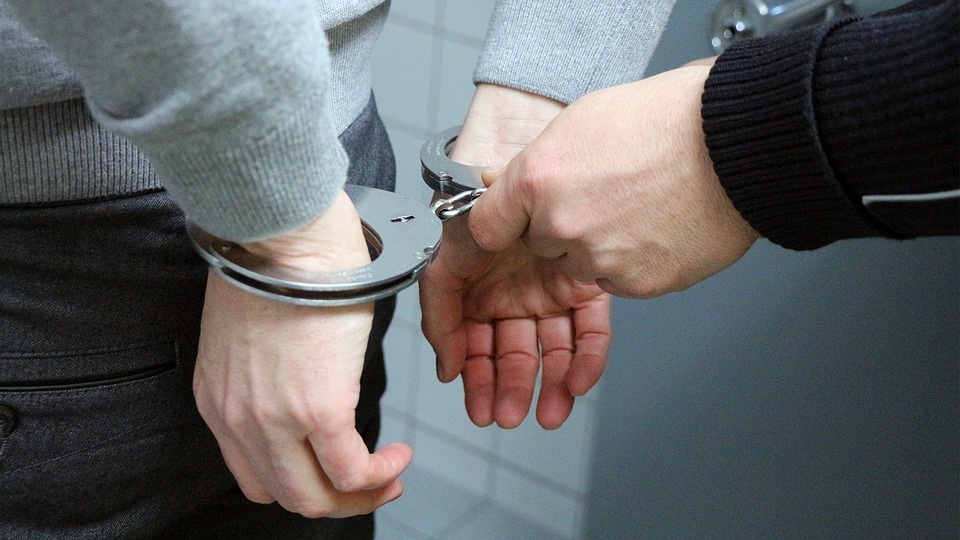
\includegraphics[width=300px]{223.jpg}%
\newline%
%
Bogotá.{-} El canciller de Colombia, Carlos Holmes Trujillo, denunció este miércoles el "aterrador silencio" del gobierno de Venezuela frente al reclamo diplomático por la "detención arbitraria" de 59 colombianos, presos desde 2016 sin fórmula de juicio.%
\newline%
%
"Se han mandado 94 notas (de protesta). El silencio del gobierno venezolano es absolutamente aterrador", dijo este miércoles el ministro de Relaciones Exteriores en un evento con empresarios en Cali.%
\newline%
%
Entretanto, la cancillería informó el martes en un comunicado que envió una nota verbal a la alta comisionada de las Naciones Unidas para Derechos Humanos, Michelle Bachelet, para denunciar "una vez más" las "condiciones deplorables" en las que permanecen los colombianos detenidos en La Yaguara, desde el 1 de septiembre de 2016.%
\newline%
%
La justicia de Venezuela los acusa de terrorismo, asociación para delinquir y falsificación de documentos, delitos que Bogotá niega.%
\newline%
%
Según el cónsul de Colombia en Caracas, Juan Carlos Pérez, una jueza había dictaminado en pasados días su libertad "porque no encontró pruebas de que fueran paramilitares o que planearan matar al presidente Maduro" y agregó que el único delito que han cometido es estar indocumentados, por lo que procedería, en todo caso, la deportación.\newline%
Sin embargo, los colombianos siguen en prisión.%
\newline%
%
El director del ONG Human Right Watch (HRW), José Miguel Vivanco, afirmó que el primer dictamen fue revocado por el Tribunal Supremo {-} al que acusa de estar al servicio del Ejecutivo {-}  y describió el caso como un "secuestro".%
\newline%
%
Se trata de una "retaliación" del gobierno de Nicolás Maduro, "para protestar por la política exterior del actual presidente Iván Duque", dijo Vivanco este miércoles a medios radiales colombianos.%
\newline%
%
\end{document}